

\subsection{Lattice setup}
    Gauge configurations in this work were obtained from the ensemble A40.24 which has been generated using $N_f = 2 + 1 + 1$ quark flavors. Details can be looked up in \cite{guage_configurations}.
    
    \begin{table}[h]
        \centering
        \begin{tabular}{lllllll}
        \hline
        \multicolumn{1}{|c|}{$\#$ used configurations} & \multicolumn{1}{c|}{$\beta$} & \multicolumn{1}{c|}{$\kappa$} & \multicolumn{1}{c|}{$a\mu_I$} & \multicolumn{1}{c|}{$a\mu_\sigma$} & \multicolumn{1}{c|}{$a\mu_\delta$} & \multicolumn{1}{c|}{$(L/a)^3 \times T$} \\ \hline
        \multicolumn{1}{|c|}{11} & \multicolumn{1}{c|}{3.9} & \multicolumn{1}{c|}{0.160856} & \multicolumn{1}{c|}{0.0040} & \multicolumn{1}{c|}{??} & \multicolumn{1}{c|}{??} & \multicolumn{1}{c|}{$24^3 \times 48$} \\ \hline
                               &                       &                       &                       &                       &                       &                       \\
                               &                       &                       &                       &                       &                       &                      
        \end{tabular}
        \caption{Parameters of gauge configurations used}
        \label{table_gauge_params}
    \end{table}
    % TODO explanation
    
\subsection{Meson masses}
    To investigate the accuracy and usefulness of the method of distillation described in this thesis comutations of charmonium state correlation functions where performed. These enable one to test different configurations of eigenvectors in relatively short times compared to the use of light doublet states. Beside the number of gauge configurations the number of eigenvectors can be arbitrarily set. In this section I will present the results for 2, 5 and 10 eigenvectors on the 11 gauge configurations mentioned in the previous section.\\
    
    In all computations the following creation operator was used:
    \begin{equation}
        \Operator(t) = \bar{\chi}^{(c)}(t)\gamma_5\chi^{(c)}(t)
    \end{equation}
    Therefore the resulting meson has quantum numbers $0(0^-)$

    \begin{figure}[H]
    \centering
    \begin{minipage}{0.5\textwidth}
        \centering
        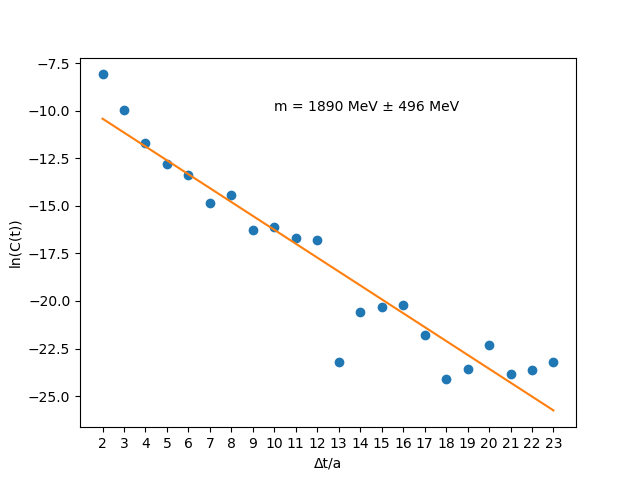
\includegraphics[width=1\textwidth]{images/Log_1ev.png} % first figure itself
        \caption{first figure}
    \end{minipage}\hfill
    \begin{minipage}{0.5\textwidth}
        \centering
        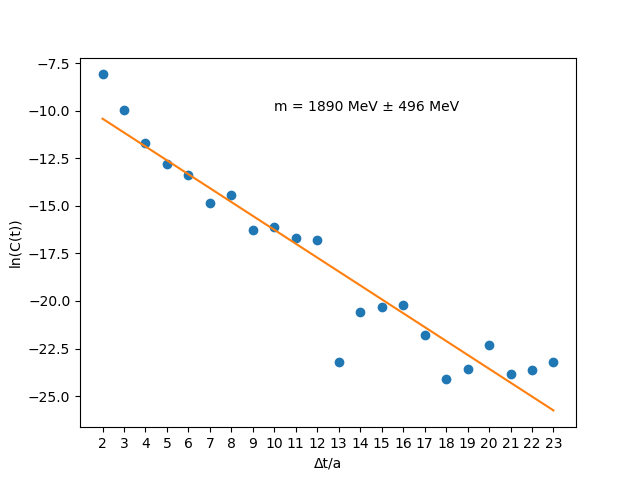
\includegraphics[width=1\textwidth]{images/Log_1ev.png} % second figure itself
        \caption{second figure}
    \end{minipage}
\end{figure}
    \begin{figure}[H]
    \centering
        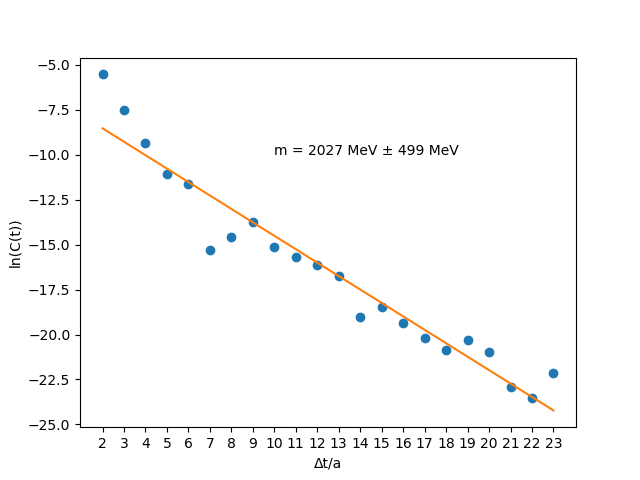
\includegraphics[width=1\textwidth]{images/Log_5ev.png} % first figure itself
\end{figure}